\pageIconSecurity
\ainfoX{Clément Aubert and Neea Rusch}{In review at \href{https://fscd2025.github.io}
{FSCD 2025: Formal Structures for Computation and Deduction}}{}
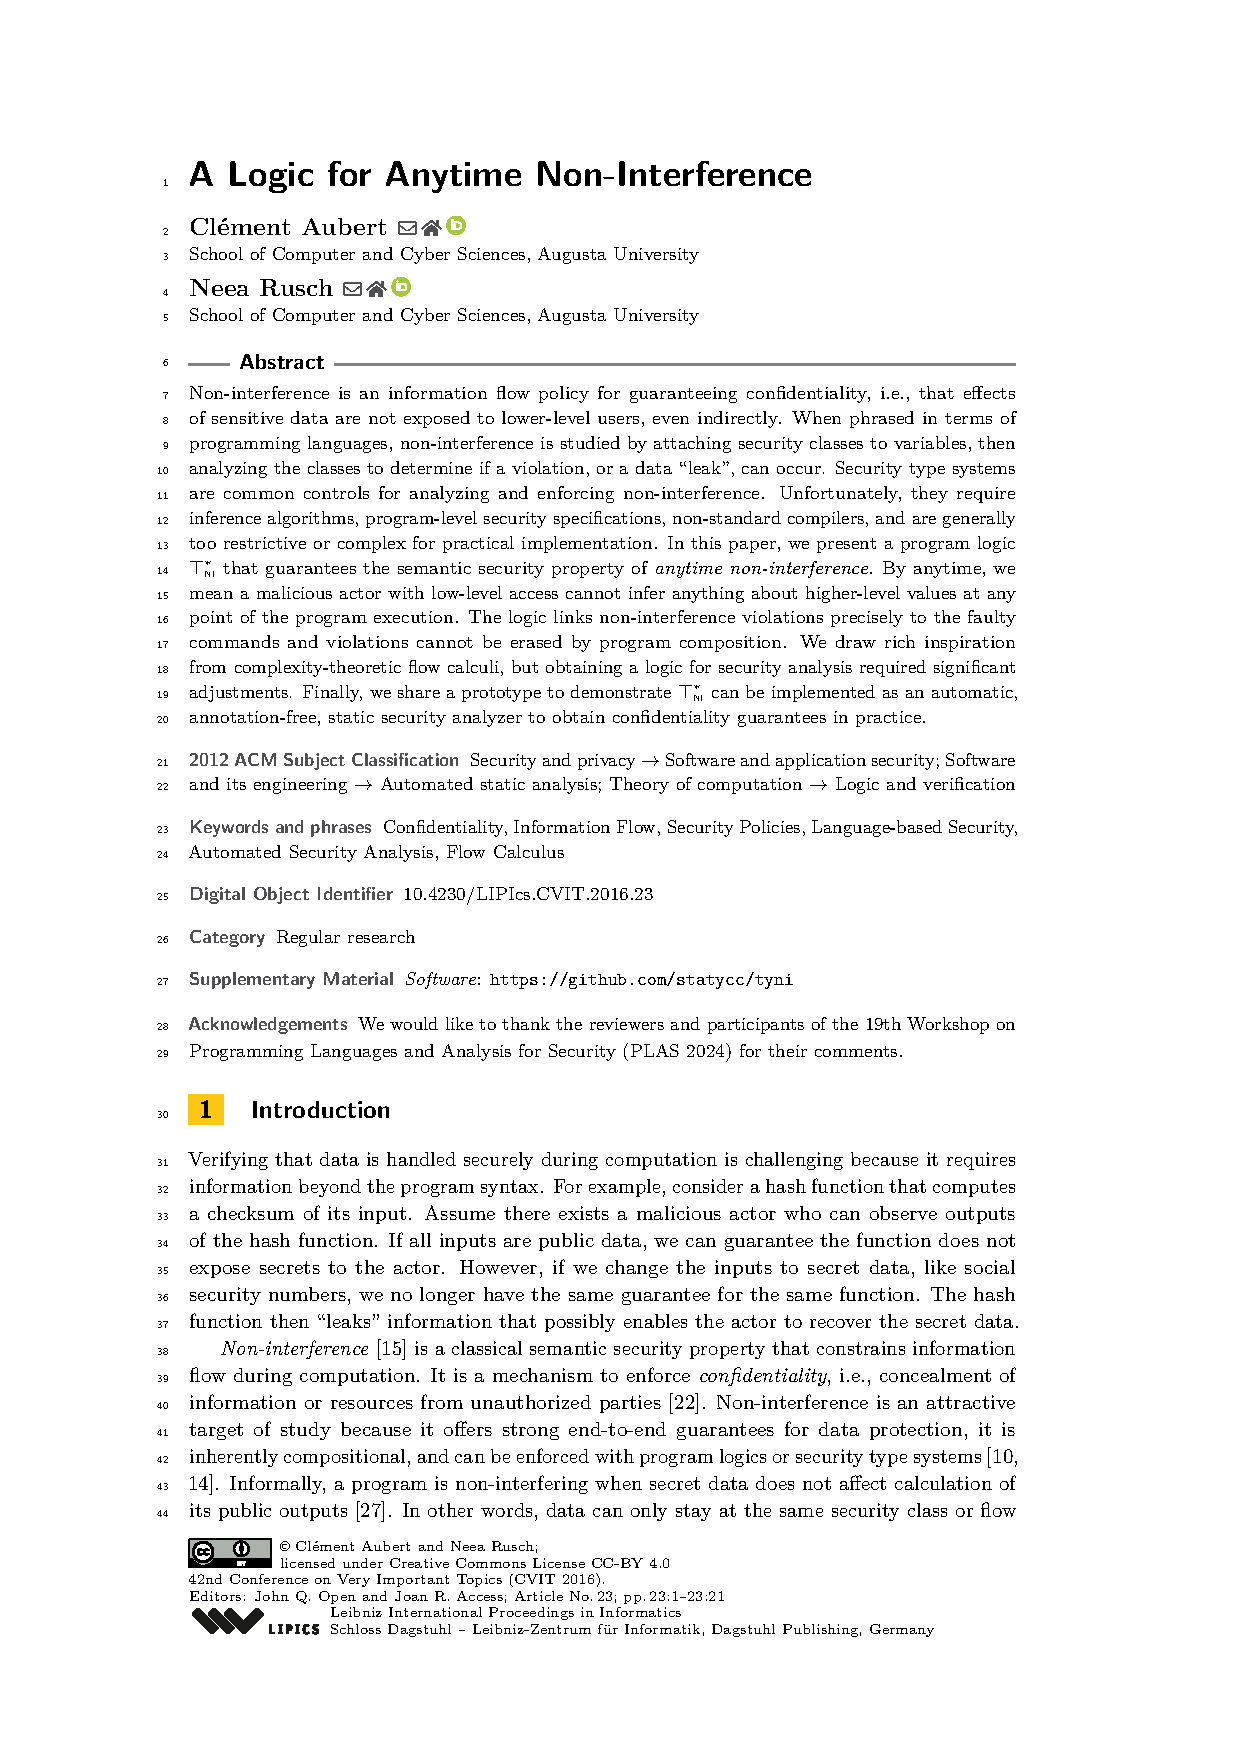
\includepdf[pages={1-},addtotoc={
    1,subsection,2,Introduction,sec:introduction,
    4,subsection,2,High-level Overview,sec:overview,
    4,subsection,2,The Non-interference Logic,ni-logic,
    9,subsection,2,Capturing Anytime Non-Interference,sec:at-soundness,
    10,subsection,2,Interpreting Function Calls in an Anytime Non-Interfering Context,sec:fct-calls,
    13,subsection,2,Practical Applications and Comparison,sec:apps,
    15,subsection,2,{Conclusion: Strengths, Limitations and Future Directions},sec:conclusion,
    18,subsection,2,{Appendix A: Proof of Thm. 16},sec:app-a,
    19,subsection,2,{Appendix B: Examples},sec:app-b},
    addtolist={
        5,figure,{A Simple Imperative while Language},fig:grammar,
        5,table,{Definition of Out, In and Occ for commands},table:ni-def-out-in-occ,
        7,figure,{Statement Examples, Sets, Representations of Possible Violation(s)},fig:ni-dependences,
        7,figure,{Security-Flow Matrix of Compositions},fig:ni-composition,
        12,figure,{Statement Examples, Interpretation and Sets -- Involving Effects},fig:fct-effect},
    pagecommand={\thispagestyle{empty}%
    \addtoindex{Dependency Core Calculus}{15}
    \addtoindex{Hasse diagram}{20}
    \addtoindex{Hasse diagram}{3}
    \addtoindex{Hasse diagram}{6}
    \addtoindex{Polybench/C}{21}
    \addtoindex{Rice's Theorem}{2}
    \addtoindex{attacker (adversary)}{13}
    \addtoindex{attacker (adversary)}{3}
    \addtoindex{attacker (adversary)}{7}
    \addtoindex{attacker (adversary)}{9}
    \addtoindex{attacker model!program centric}{3}
    \addtoindex{attacker model}{3}
    \addtoindex{bytecode}{13}
    \addtoindex{bytecode}{14}
    \addtoindex{complexity class}{15}
    \addtoindex{confidentiality}{14}
    \addtoindex{confidentiality}{1}
    \addtoindex{declassification}{15}
    \addtoindex{dependency analysis}{15}
    \addtoindex{dependency analysis}{5}
    \addtoindex{dynamic code loading}{2}
    \addtoindex{matrix!hollow}{19}
    \addtoindex{matrix!hollow}{5}
    \addtoindex{matrix!hollow}{6}
    \addtoindex{imperative programs}{15}
    \addtoindex{imperative programs}{3}
    \addtoindex{imperative programs}{4}
    \addtoindex{information flow!control}{3}
    \addtoindex{information flow!explicit}{2}
    \addtoindex{information flow!explicit}{4}
    \addtoindex{information flow!implicit}{15}
    \addtoindex{information flow!implicit}{2}
    \addtoindex{information flow!implicit}{4}
    \addtoindex{information flow!implicit}{8}
    \addtoindex{information flow!policy}{14}
    \addtoindex{information flow!policy}{15}
    \addtoindex{information flow!policy}{1}
    \addtoindex{information flow!policy}{20}
    \addtoindex{information flow!policy}{21}
    \addtoindex{information flow!policy}{3}
    \addtoindex{information flow!policy}{6}
    \addtoindex{information flow}{14}
    \addtoindex{information flow}{19}
    \addtoindex{information flow}{1}
    \addtoindex{information flow}{21}
    \addtoindex{information flow}{2}
    \addtoindex{information flow}{3}
    \addtoindex{intermediate representation}{14}
    \addtoindex{language-based security}{14}
    \addtoindex{language-based security}{15}
    \addtoindex{language-based security}{2}
    \addtoindex{lattice}{3}
    \addtoindex{matrix!empty}{7}
    \addtoindex{monoid}{5}
    \addtoindex{monoid}{6}
    \addtoindex{monoid}{8}
    \addtoindex{non-interference!anytime}{10}
    \addtoindex{non-interference!anytime}{12}
    \addtoindex{non-interference!anytime}{13}
    \addtoindex{non-interference!anytime}{14}
    \addtoindex{non-interference!anytime}{15}
    \addtoindex{non-interference!anytime}{18}
    \addtoindex{non-interference!anytime}{19}
    \addtoindex{non-interference!anytime}{1}
    \addtoindex{non-interference!anytime}{20}
    \addtoindex{non-interference!anytime}{21}
    \addtoindex{non-interference!anytime}{2}
    \addtoindex{non-interference!anytime}{3}
    \addtoindex{non-interference!anytime}{8}
    \addtoindex{non-interference!anytime}{9}
    \addtoindex{non-interference!progress-sensitive}{2}
    \addtoindex{non-interference!termination-insensitive}{2}
    \addtoindex{non-interference}{10}
    \addtoindex{non-interference}{13}
    \addtoindex{non-interference}{14}
    \addtoindex{non-interference}{15}
    \addtoindex{non-interference}{18}
    \addtoindex{non-interference}{19}
    \addtoindex{non-interference}{1}
    \addtoindex{non-interference}{2}
    \addtoindex{non-interference}{3}
    \addtoindex{non-interference}{4}
    \addtoindex{non-interference}{5}
    \addtoindex{non-interference}{8}
    \addtoindex{non-interference}{9}
    \addtoindex{security class}{10}
    \addtoindex{security class}{11}
    \addtoindex{security class}{13}
    \addtoindex{security class}{14}
    \addtoindex{security class}{15}
    \addtoindex{security class}{1}
    \addtoindex{security class}{2}
    \addtoindex{security class}{3}
    \addtoindex{security class}{4}
    \addtoindex{security class}{5}
    \addtoindex{security class}{6}
    \addtoindex{security class}{7}
    \addtoindex{security class}{8}
    \addtoindex{security class}{9}
    \addtoindex{security objective}{3}
    \addtoindex{security type system}{15}
    \addtoindex{security type system}{1}
    \addtoindex{security type}{15}
    \addtoindex{security type}{3}
    \addtoindex{matrix!security-flow}{11}
    \addtoindex{matrix!security-flow}{14}
    \addtoindex{matrix!security-flow}{21}
    \addtoindex{matrix!security-flow}{4}
    \addtoindex{matrix!security-flow}{5}
    \addtoindex{matrix!security-flow}{6}
    \addtoindex{matrix!security-flow}{7}
    \addtoindex{side effect}{10}
    \addtoindex{side effect}{12}
    \addtoindex{side effect}{13}
    \addtoindex{side effect}{2}
    \addtoindex{side effect}{3}
    \addtoindex{system model}{3}
    \addtoindex{termination}{14}
    \addtoindex{termination}{2}
    \addtoindex{termination}{9}
    }]{pdf/pubs_ni.2025.pdf}